\documentclass[11pt]{article}

\usepackage[italian]{babel}
\usepackage[utf8]{inputenc}  
\usepackage{amsmath}         
\usepackage{amssymb}         
\usepackage{graphicx}        
\usepackage{geometry}        
\usepackage{fancyhdr}            
\usepackage{float} 
\usepackage{xcolor}
\usepackage{tabularx}
\usepackage{multicol}
\usepackage{caption}
\usepackage{tcolorbox} % Pacchetto per la nota evidenziata

% Impostazioni per i margini
\geometry{a4paper, margin=0.8in}

% Grandezza righe tabelle
\renewcommand{\arraystretch}{1.2} % Aumenta l'altezza delle righe

% Intestazioni
\pagestyle{fancy}
\fancyhf{}
\fancyhead[L]{Linguaggi Formali e Compilatori}
\fancyhead[R]{Soluzione Esercizi Tipo - Parte I}
\fancyfoot[C]{\thepage}   
\setlength{\headheight}{14pt}

\begin{document}
%%%%%%%%%%%%%%%%%%%%%%% ESERCIZIO 1 %%%%%%%%%%%%%%%%%%%%%%%
\section*{Esercizio 1}
A lezione non è stata fatta la dimostrazione, ma si può dimostrare
che se due linguaggi sono regolari allora la loro unione è regolare, quindi la risposta è \textbf{VERO}.
%%% Nota inizia qui %%%
\begin{tcolorbox}[colframe=orange!70!black, colback=orange!10!white, title=\textbf{\textit{Nota inutile ai fini dell'esercizio:}}]
Se prendessimo ad esempio:
\begin{itemize}
  \item ${\cal L}_1 = \{w \in \{a,b\}^*|\;w\;ha\;una\;lunghezza\;pari\}$  
  \item ${\cal L}_2 = \{w \in \{a,b\}^*|\;w\;termina\;con\;a\}$  
\end{itemize}
\begin{multicols}{2}
  \begin{figure}[H]
  \centering
    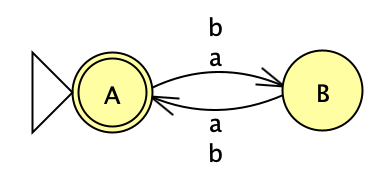
\includegraphics[height=2.5cm]{img/01Pari.png}
    \label{fig:01-DFA-pari}
    \caption*{DFA per ${\cal L}_1$}
  \end{figure}
  \begin{figure}[H]
  \centering
    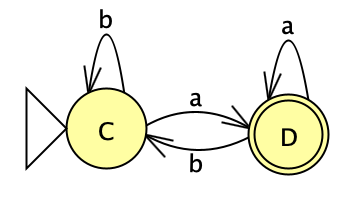
\includegraphics[height=2.5cm]{img/01FinisceConA.png}
    \label{fig:01-DFA-finisce-con-a}
    \caption*{DFA per ${\cal L}_2$}
  \end{figure}
\end{multicols}
L'unione di  ${\cal L}_1$ con  ${\cal L}_2$ sta a significare che la 
parola su $\{a, b\}$ deve essere pari oppure finire con la lettera $a$.
Per costruire l'automa che verifichi l'unione potremo leggere la parola
contemporaneamente in entrambi i DFA e se al termine della parola mi 
trovo in uno stato finale di uno dei due DFA allora la parola appartiene
all'unione.

Possiamo costruire il DFA finale quindi facendo il prodotto cartesiano
degli stati, quello iniziale sarà $AC$ mentre quelli finali saranno 
$AC$, $AD$ e $BD$ ottenendo il seguente DFA, confermando che l'unione 
è regolare.
\begin{figure}[H]
  \centering
  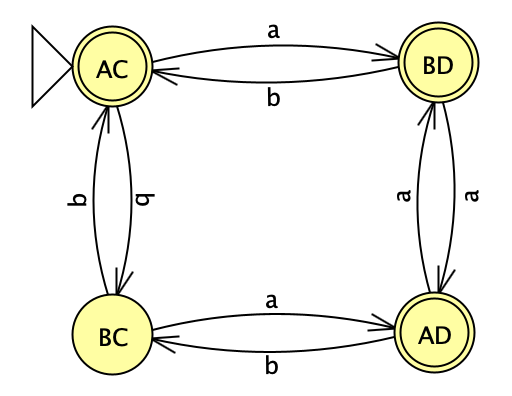
\includegraphics[height=4.3cm]{img/01Unione.png}
  \label{fig:01-DFA-unione}
\end{figure}
\noindent Andando ad 'occhio' si poteva comunque costruire un DFA 
che riconosceva ${\cal L}_1 \cup {\cal L}_2$:
\begin{figure}[H]
  \centering
  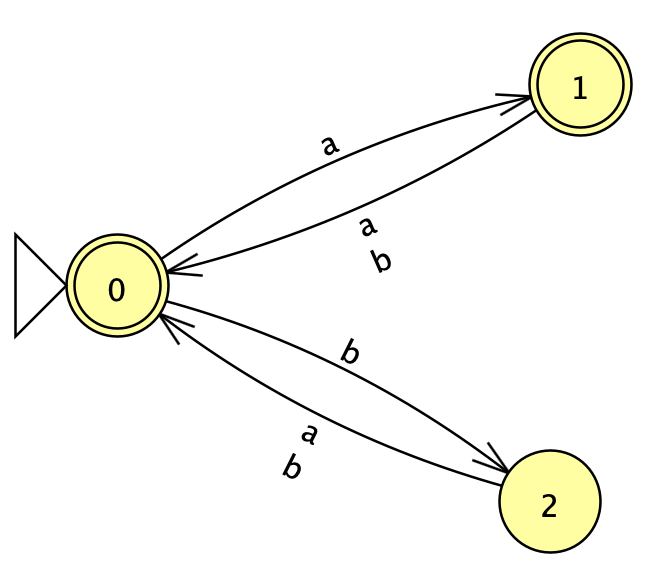
\includegraphics[height=4.3cm]{img/01Unione-1.png}
  \label{fig:01-DFA-unione-1}
\end{figure} 
\end{tcolorbox}
%%% Nota finisce qui %%%
%%%%%%%%%%%%%%%%%%%%%%% ESERCIZIO 2 %%%%%%%%%%%%%%%%%%%%%%%
\section*{Esercizio 2}
Sulle slide o dispensa studenti.
\newpage
%%%%%%%%%%%%%%%%%%%%%%% ESERCIZIO 3 %%%%%%%%%%%%%%%%%%%%%%%
\section*{Esercizio 3}
Per la costruzione di un DFA partendo da un NFA partiamo dallo
stato iniziale $A$ e calcoliamo la sua $\epsilon$-chiusura:
$$closure(A) = \{A\;,B,\;C,\;E\} = T_0$$
Da questo stato controlliamo in che stati andiamo a finire tramite
una 
\begin{itemize}
  \item a-transizione: $closure(D,\;E) = \{D,\;E\} = T_1$
  \item b-transizione: $closure(A,\;E) = \{A\;,B,\;C,\;E\} = T_0$
\end{itemize}
Facciamo la stessa cosa da $T_1$:
\begin{itemize}
  \item a-transizione: $closure(E) = \{E\} = T_2$
  \item b-transizione: $closure(A,\;B) = \{A\;,B,\;C,\;E\} = T_0$
\end{itemize}
Facciamo la stessa cosa da $T_2$:
\begin{itemize}
  \item a-transizione: $closure(E) = \{E\} = T_2$
  \item b-transizione: $closure(A) = \{A\;,B,\;C,\;E\} = T_0$
\end{itemize}
La funzione di transazione del DFA sarà:
\begin{table}[H]
  \centering
  \begin{tabularx}{\textwidth}{|>{\centering\arraybackslash}X|>{\centering\arraybackslash}X|>{\centering\arraybackslash}X|}
  \hline
  & \textbf{a} & \textbf{b}  \\
  \hline
  $T_0$ & $T_1$ & $T_0$\\
  \hline
  $T_1$ & $T_2$ & $T_0$ \\
  \hline
  $T_2$ & $T_2$ & $T_0$ \\
  \hline
  \end{tabularx}
  \label{tab:03-parsing-table}
\end{table}
Quindi se $Q$ è lo stato iniziale del DFA allora: $Q[ab] = T_0 = {A, B, C, E}$
\begin{figure}[H]
  \centering
  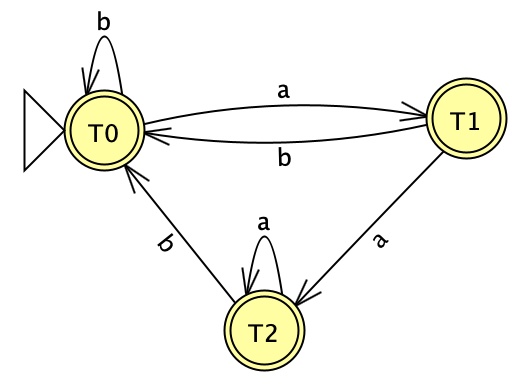
\includegraphics[height=4.3cm]{img/03DFA.png}
  \label{fig:03-DFA}
\end{figure} 
\end{document}
